\documentclass[a4paper,10pt,twoside]{article}

%===========PACOTES
\usepackage[body={170mm,235mm}]{geometry}
%\usepackage[portuguese]{babel}
\usepackage{a1}
\usepackage[english]{babel}
\usepackage[latin1]{inputenc} %permite o uso de acentos
%\usepackage[dvips]{color}
\usepackage{amsfonts,amssymb}
%\usepackage{epsfig}
\usepackage{amsmath}
\usepackage{graphicx}	

% makeidx
\usepackage{makeidx}
% make index
\makeindex
%\usepackage[pdftex]{graphicx}


\def\mapright#1#2#3{\smash{\mathop{\hbox to
#3{\rightarrowfill}}\limits^{#1}_{#2}}}

\def\mapleft#1#2#3{\smash{\mathop{\hbox to
#3{\leftarrowfill}}\limits^{#1}_{#2}}}

\def\mapright#1#2{\smash{\mathop{\hbox to 0.90cm{\rightarrowfill}}\limits^{#1}_{#2}}}
\def\mapleft#1#2{\smash{\mathop{\hbox to 0.90cm{\leftarrowfill}}\limits^{#1}_{#2}}}

\def\mapleftright#1#2{\smash{\mathop{\hbox to 0.80cm{\leftarrowfill \rightarrowfill}}\limits^{#1}_{#2}}}
\def\ext{\times \! \vrule depth0pt height5pt width0.35pt}

\def\H{\mathcal H}
\def\D{\mathcal D}
\def\B{\mathcal B}
\def\C{\mathbb C}
\def\R{\mathbb R}
\def\S{\mathbb S}
\def\U{\mathcal U}
\def\Z{\mathbb Z}

\title{Closed oriented 3-manifolds are equivalence classes of plane graphs
\footnote{2010 Mathematics Subject Classification: 
05C85 and 05C83 (primary), 57M27 and 57M15 (secondary)}} 
\author{S�stenes L. Lins}

\date{\today}


\begin{document}


\maketitle

\begin{abstract}
A {\em blink} is a plane graph with an arbitrary bipartition of its edges.
As a consequence of a recent result of Martelli, we show that the homeomorphisms classes
of closed oriented 3-manifolds are in 1-1 correspondence with classes of blinks. Two blinks
are equivalent if they are linked by a finite sequence of local moves, where each move
is one of a concrete list of 64 moves: they organize in 8 types,
each beeing essentlially the same move on 8 simply related configurations. 
The size of the list can be substantially
decreased at the cost of loosing symmetry.
\end{abstract}


\section{Introduction: knots, links, 3-manifolds and Martelli's moves}
In a recent paper B. Martelli \cite{martelli2012finite} presented a reformulation of
the Fenn-Rourke version (\cite{fenn1979kirby}) of Kirby's calculus \cite{kirby1978calculus}.
Our objective here is to further reformulate Martelli's moves so as to obtain a calculus
of blinks, which is an exact combinatorial counterpart for factorizing homeomorphisms of
closed orientable 3-manifolds. This goal is desirable because it has the consequence that each 3-manifold
become a subtle class of plane graphs. Our exposition is complete and elementary seeking
to reach both audiences: topologists and combinatorialists.

A {\em knot} is an embedding of a circle, an $\mathbb{S}^1$, into $\mathbb{R}^3$ or  $\mathbb{S}^3$.
A {\em link with $k$ components} is an embedding of a disjoint union of $k$ copies of $\mathbb{S}^1$
into $\mathbb{R}^3$ or  $\mathbb{S}^3$. In this way, a knot is a link with one component.

Knots and links can be presented by their {\em decorated 
general position projections} into a fixed plane $\mathbb{R}^2$. {\em General position} means that 
in the image of the link there is no triple points and that at each neighborhood of
each double is the transversal crossing of two segments of the link, named {\em strands}. 
{\em Decorated} means that we keep the information
of which strand is the upper one, usually by removing a piece of the lower strand. In this paper
we use another way to decorate the link projections: the images of the link components are thich black curves
and the upper strands are indicated by a thinner white segment inside the thich black curve at the crossing.


\begin{figure}[!h]
\begin{center}
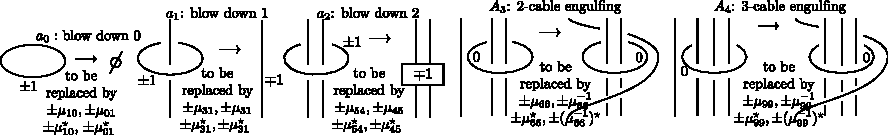
\includegraphics[width=16.5cm]{A.figs/Martelli.pdf} 
\caption{\sf Martelli's calculus on fractional framed links}
\label{fig:blinklinkgem}
\end{center}
\end{figure} 

\begin{figure}[!h]
\begin{center}
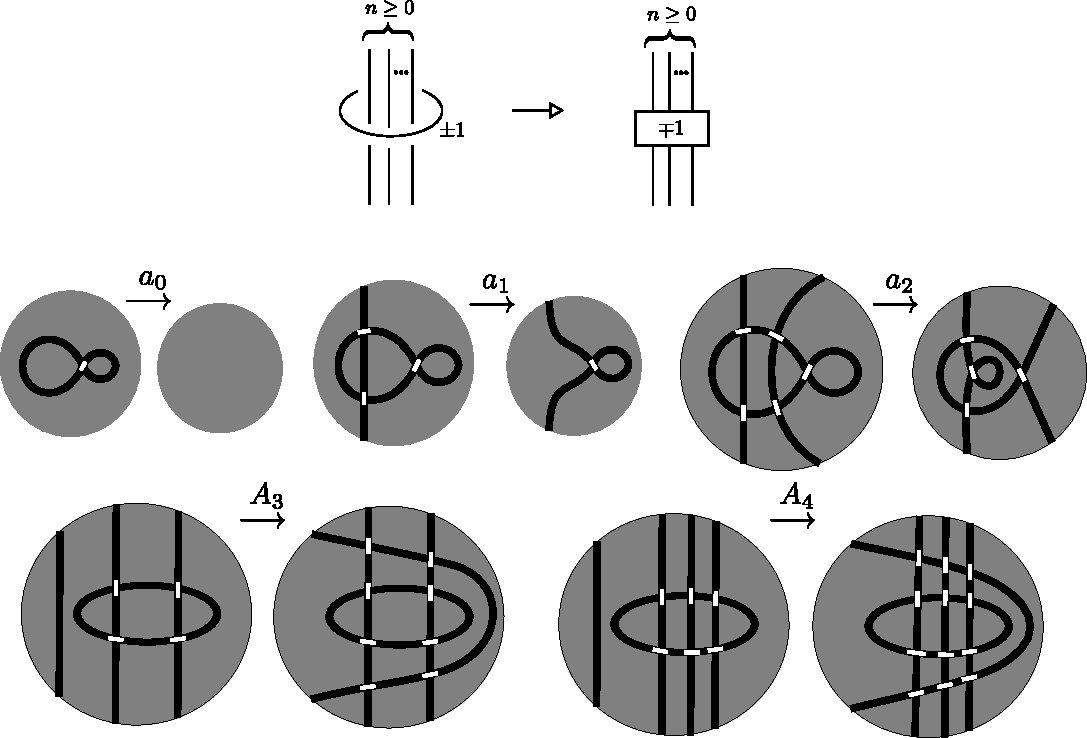
\includegraphics[width=13.5cm]{A.figs/FennRourkeMartelliBlackboard.pdf} 
\caption{\sf Fenn-Rourke infinite 1-parametrized blown-down moves 
and Martelli's moves in blackboard framed form}
\label{fig:FennRourkeMartelliBlackboard}
\end{center}
\end{figure} 

\begin{figure}[!h]
\begin{center}
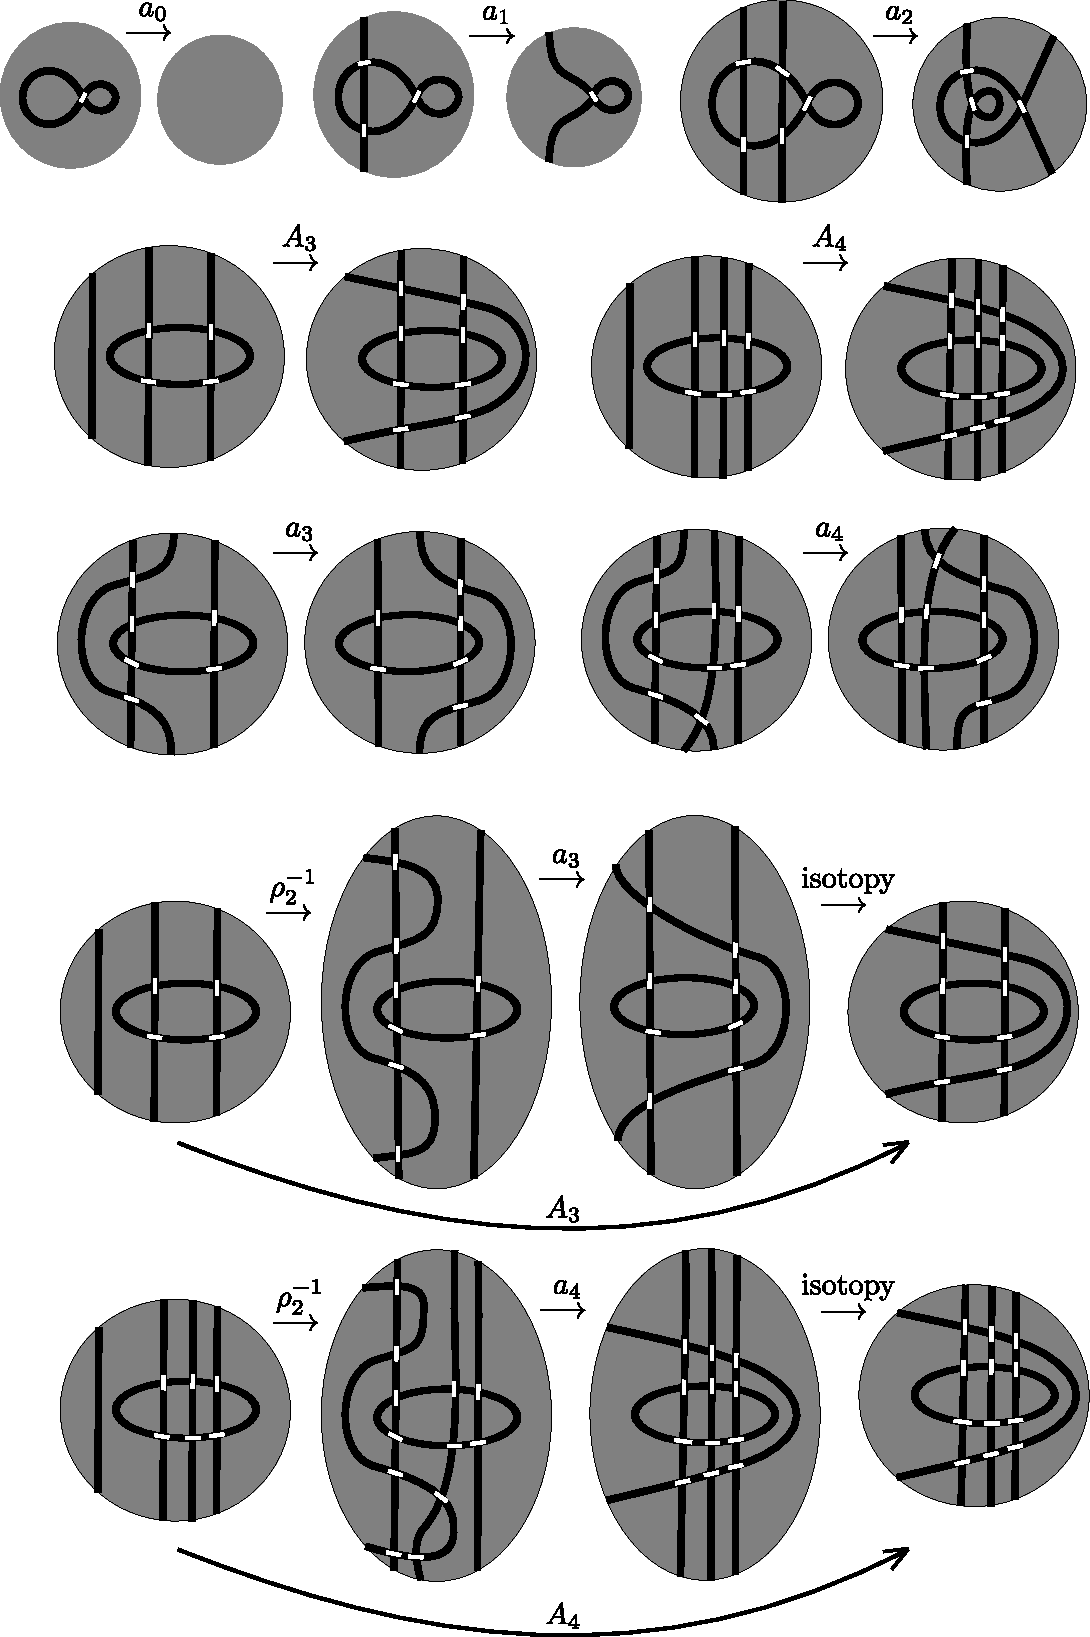
\includegraphics[width=11cm]{A.figs/MartelliReformulationLinks.pdf} 
\caption{\sf The minimum blink, minimum link and minimum gem inducing the binary tetrahedral space}
\label{fig:blinklinkgem}
\end{center}
\end{figure} 

\begin{figure}[!h]
\begin{center}
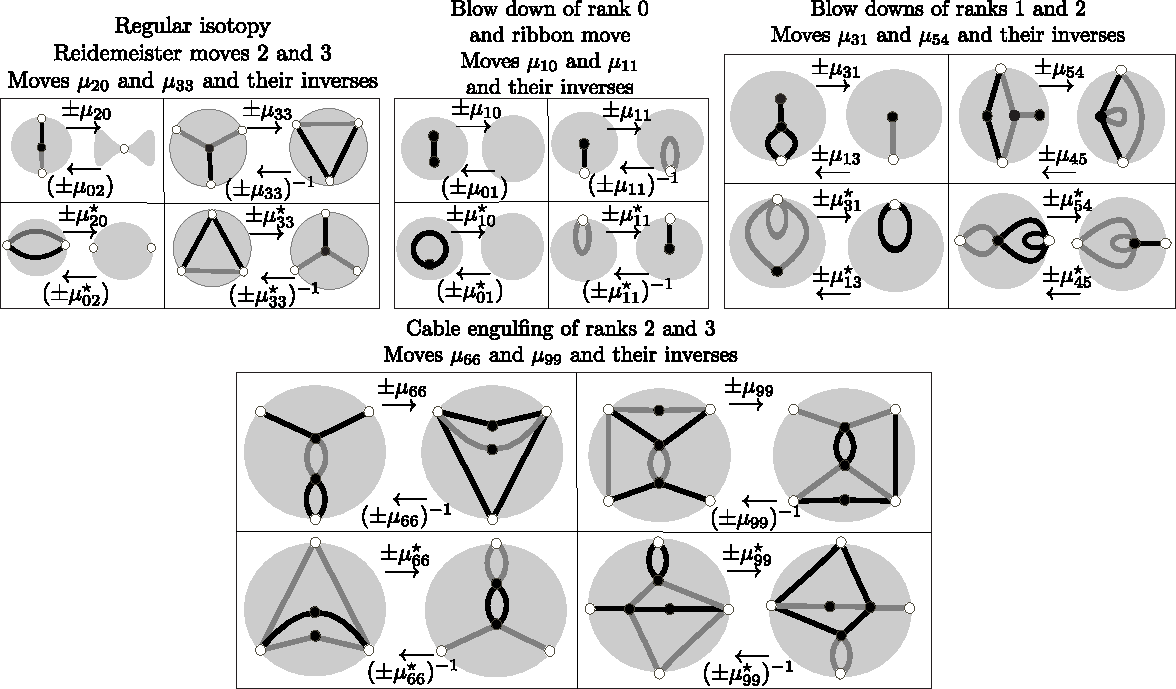
\includegraphics[width=11cm]{A.figs/blinkcalculus.pdf} 
\caption{\sf Blink-coin reformulation of Martelli's moves}
\label{fig:blinkcalculus}
\end{center}
\end{figure} 




% \begin{figure}[!h]
% \begin{center}
% \includegraphics[width=12.5cm]{A.figs/seconddoubtB.pdf}
% \caption{\sf Finding presentations for the fundamental groups of $M^ 3[2125]$ and $M^ 3[2165]$}
% \label{fig:seconddoubtB}
% \end{center}
% \end{figure}

%-----------------------------------
\bibliographystyle{plain}
%\bibliographystyle{is-alpha}
%\addcontentsline{toc}{bibliografia}{\MakeTextUppercase{Refer�ncias Bibliogr�ficas}}
%\bibliography{d:/slsl\3.DadosSostenes.35.ArtigosLivros.bibtexGoogleScholar/bibtexIndex.bib} % bib file is slsl.bib
%\bibliography{~/home/ricardo/Dropbox/35.ArtigosLivros.bibtexGoogleScholar/bibtexIndex.bib}
\bibliography{bibtexIndex.bib}
%\bibliography{slsl}


\vspace{5mm}
\begin{center}
\hspace{7mm}
\begin{tabular}{l}
   S\'ostenes L. Lins\\
   Centro de Inform\'atica, UFPE \\
   Av. Jornalista Anibal Fernandes s/n\\
   Recife, PE 50740-560 \\
   Brazil\\
   sostenes@cin.ufpe.br
\end{tabular}


\end{center}


\end{document}

\begin{figure}[!htb]
\begin{center}
\includegraphics[scale=0.8]{A.figs/seconddoubt.pdf}
\caption{Are these 3-manifolds homeomorphic?}
\label{fig:seconddoubt}
\end{center}
\end{figure}

% \printindex
